\part{Recherche Opérationnel}
\pagebreak

\chapter{Rappel}
\section{Pivot de gauss}

$ L1 et L2 =
\begin{cases}
L1: 160 = 8x + 4y\\
L2: 120 = 4x + 6y 
\end{cases}$
\\
$( L2*(-2) )=
\begin{cases}
L1: 160 = 8x + 4y\\
L2: -240 = -8x -12y
\end{cases}$
\\
$( L2=L2+L1 )=
\begin{cases}
L1: 160 = 8x + 4y\\
L2: -80 = -8y
\end{cases}$
\\
$y = 10$
\\\\
$8x + 4*10 = 160$\\
$8x + 40 = 160$\\
$8x = 120$\\
$x = 15$\\

\chapter{Introduction à la PL}

Construire une modèle linéaire, c'est donc:
\begin{description}
\item[identifier] les variables de décision du problème
\item[déterminer]: la fonction objectif du modèle
\item[déterminer]: les contraintes du modèle 
\end{description}

\section{Modèle linéaire continus à 2 variables}
Soit le modèle linéaire suivantes:
\begin{description}
\item[Déterminer] $(x,y) \in \Im^2$
\item[Minimisant] $z = 1000x + 1200y$
\item[sous les contraintes]:
\begin{description}
\item[] $(1) 8x + 4y \leq 160$
\item[] $(2) 4x + 6y \leq 120$
\item[] $(3) x \leq 34$
\item[] $(4) y \leq 14$
\item[] $(5) 0 \leq x$
\item[] $(6) 0 \leq y$
\end{description}
\end{description}

\subsection{Recherche de solutions}
Après avoir tracé graphiquement tout les points:\\
Pour chaque contrainte, tracer la droite et repérer le demi plan des solution: exemple pour (5) et (6), x et y doivent être supérieurs ou égal à 0, d'où le demi plan des solution sont toutes les valeurs positives.\\
La partie En vert représente la région admissible, quelque soit le point choisis dans ce vert, aucune contrainte ne sera violé.\\
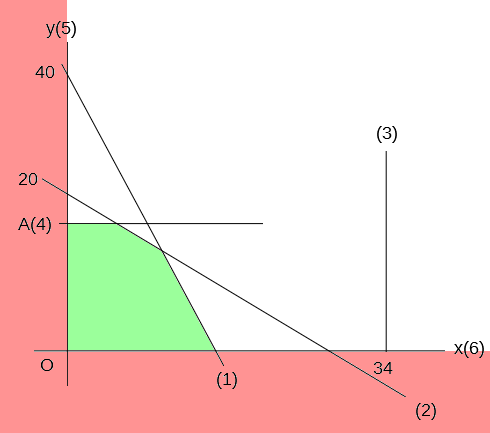
\includegraphics[scale=0.55]{img/ro-pl-2var_0.png} 
\subsection{recherche de la solution optimal}

Changer l'équation $z$ tel que $z$ soit égal à $0$
\begin{description}
\item[$z$] = $1000x + 1200y$ = $0$ = $1000*(1200) + 1200 *(-1000)$
\end{description}
Traçons la droite $(0,0)$, $(1200,-1000)$
\begin{description}
\item[Un point extrême]: est un point se trouvant sur l'intersection de 2 contraintes et étant dans la zone admissible.
\item[L'altitude]: est la droite (rouge) la plus haute touchant un point extrême, ce point sera le vecteur $(x,y)$ le plus optimal pour $z$.
\item[] Les droites rouges doivent être toutes parallèles.
\end{description}
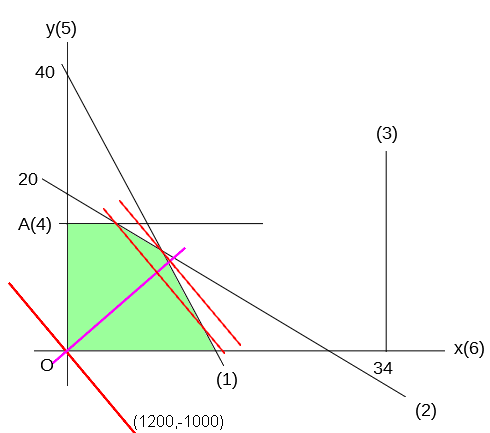
\includegraphics[scale=0.55]{img/ro-pl-2var_1.png} \\
Dans cette exemple le point (15,10) est le point extrême maximal pour l'équation z.\\
\pagebreak
\chapter{Le simplexe}
Soit le modèle linéaire suivantes:
\begin{description}
\item[Déterminer] $(x,y) \in \Im^2$
\item[Maximisant] $Z = 3x + 7y$
\item[sous les contraintes]:
\begin{description}
\item[] (1) $ -x + y \leq 3$
\item[] (2) $ y \leq 8$
\item[] (3) $ 2x - y \leq 28$
\item[] (5) $ 0 \leq x$
\item[] (6) $ 0 \leq y$
\end{description}
\end{description}

\section{Initialisation du simplexe}
Pour chaque expression du type $(1)(2)(3)$ intégrer un $e_i$ pour la transformer en équation.\\
On appel les $e_1$ des variables d'accumulation, Ce qui fait\\
\begin{description}
\item[Déterminer] $(x,y,e_1,e_2,e_3) \in \Im^5$
\item[Maximisant] $Z = 3x + 7y$
\item[sous les contraintes]:
\begin{description}
\item[] (1) $ -x + y + e_1 = 3$
\item[] (2) $ y + e_2 = 8$
\item[] (3) $ 2x - y + e_3 = 28$
\item[] (5) $ 0 \leq x$
\item[] (6) $ 0 \leq y$
\item[] (7) $ e_1,e_2,e_3 \geq 0$
\end{description}
\end{description}

\section{Canonicité du modèle}
Soit les valeurs (pour la première itération)
\begin{description}
\item[Hors Base] $(x,y)$
\item[Base] $(e_1,e_2,e_3)$
\end{description}

Un modèle est canonique que si:
\begin{description}
\item[si toutes les variables de Base] ne sont pas dans Z.
\end{description}

\section{Solution admissible}
\begin{description}
\item[] (1) $-x + y + e_1 = 3$
\item[] (2) $x - e_1 + e_2 = 5$
\item[] (3) $3x - e_1 + e_3 = 25$
\item[Variable hors base] = $x,e_1$
\item[Variable Base] = $y,e_2,e_3$
\item[Avec comme solution admissible] $A\ Deduire (x,y,e_1,e_2,e_3)$
\end{description}
\ \\
Pour toute variable présente dans l'ensemble $Hors\ base$ la valeur admissible est égal à $0$\\
Donc solution admissible = $(0, y, 0, e_2, e_3)$\\
Les 3 dernières valeurs sont les résultat des équations (soit $3$, $5$ et $25$).\\
Pour chaque équation nous lisons les termes de droit à gauche et ignorons ceux qui sont dans l'ensemble $Hors\ Base$:\\
Donc solution admissible = $(0, 3, 0, 5, 25)$\\

\section{Exemple simple Premier itération}
\subsection{Choix de la variable entrante}
$(x,y)$ sont deux choix possible, le tout est de choisir une bonne heuristique, comme celle du meilleur gain marginale, ou via la comparaison (en mode graphique):\\
$Y$ sera choisit, donc $Y$ sera notre variable entrante.\\

\subsection{Choix de la variable sortante}
Pour chaque résultat d'équation, le diviser par sa valeur de $Y$ (devant être positif (car $Y$ est la variable entrante)\\

\begin{description}
\item[] $ -x + y + e_1 = 3$ donne $\frac{3}{\crouge{1}} = 3$ (1 car $y$ = $1*y$)
\item[] $ y + e_2 = 8$ donne $\frac{8}{1} = 8$
\item[] $ 2x - y + e_3 = 28$ donne $\frac{28}{1} = 28$
\end{description}
Prendre le minimum des variables, donc se sera $3$.\\
la variable présente dans la Base sera prise comme variable sortante, dans notre cas $e_1$.\\
\pagebreak
\subsection{pivotage}
On choisis l'équation associé à la variable $e_1$ pour définir la variable entrante $y$.\\
On n'a:
\begin{description}
\item[$y$] = $\crouge{1}*(x - e_1 + 3)$
\end{description}

Puis on crée les nouvelles équations via le nouveau $y$:
\begin{description}
\item[$Z = 3x + 7y$] devient
\begin{description}
\item[$Z$] = $3x + 7(x - e_1 + 3)$
\item[$Z$] = $10x - 7e_1 + 27$
\end{description}
\item[$x - e_1 = 3$] est déjà normalisé
\item[$y + e_2 = 8$] devient
\begin{description}
\item[$8$] = $x -e_1 + 3 + e_2$
\item[$5$] = $x - e_1 + e_2$
\end{description}
\item[$2x - y + e_3 = 28$] devient
\begin{description}
\item[$28$] = $2x + (x - e_1 + 3) + e_3$
\item[$25$] = $3x - e_1 + e_3$
\end{description}
\end{description}
\subsection{Nouveau modèle}
Après cette étape nous voila avec un nouveau modèle:
\begin{description}
\item[Déterminer] $(x,y,e_1,e_2,e_3) \in \Im^5$
\item[Maximisant] $Z = 10x - 7e_1 + 21$
\item[sous les contraintes]:
\begin{description}
\item[] (1) $-x + y + e_1 = 3$
\item[] (2) $x - e_1 + e_2 = 5$
\item[] (3) $3x - e_1 + e_3 = 25$
\item[] (5) $ 0 \leq x$
\item[] (6) $ 0 \leq y$
\item[] (7) $ e_1,e_2,e_3 \geq 0$
\end{description}
\item[Variable hors base] = $x,e_1$
\item[Variable Base] = $y,e_2,e_3$
\item[Avec comme solution admissible] $(0,3,0,5,25) Z=21$
\end{description}


A ne pas oublier de vérifier la canonicité du modèle.\\

\section{Exemple simple Seconde itération}
\subsection{Choix de la variable entrante}
$X$ sera choisit, donc $X$ sera notre variable entrante.\\

\subsection{Choix de la variable sortante}
\begin{description}
\item[] $\frac{5}{\crouge{1}} = 5$
\item[] $\frac{25}{3} = 8.3$
\end{description}
Prendre le minimum des variables, donc se sera $5$, donc $e_2$.\\

\subsection{pivotage}
\begin{description}
\item[$x$] = $\crouge{1}*(e_1 - e_2 + 5)$
\end{description}

Puis on crée les nouvelles équations via le nouveau $y$:
\begin{description}
\item[$Z = 10x - 7e_1 + 27$] devient
\begin{description}
\item[$Z$] = $10(e_1 - e_2 + 5) - 7e_1 + 27$
\item[$Z$] = $3e_1 - 10e_2 + 71$
\end{description}
\item[$-x + y + e_1 = 3$] devient
\begin{description}
\item[$3$] = $-(e_1 - e_2 + 5) + y + e_1$
\item[$8$] = $y + e_2$
\end{description}
\item[$3x - e_1 + e_3 = 25$] devient
\begin{description}
\item[$25$] = $3(e_1 - e_2 + 5) -e_1 + e_3$
\item[$10$] = $2e_1 - 3e_2 + e_3$
\end{description}
\end{description}

\subsection{Nouveau modèle}
Après cette étape nous voila avec un nouveau modèle:
\begin{description}
\item[Déterminer] $(x,y,e_1,e_2,e_3) \in \Im^5$
\item[Maximisant] $Z = 3e_1 - 10x + 71$
\item[sous les contraintes]:
\begin{description}
\item[] (1) $y + e_2 = 8$
\item[] (2) $x - e_1 + e_2 = 5$
\item[] (3) $2e_1 - 3e_2 + e_3 = 10$
\item[] (5) $ 0 \leq x$
\item[] (6) $ 0 \leq y$
\item[] (7) $ e_1,e_2,e_3 \geq 0$
\end{description}
\item[Variable hors base] = $e_2,e_1$
\item[Variable Base] = $y,x,e_3$
\item[Avec comme solution admissible] $(5,8,0,0,10) Z=71$
\end{description}

A ne pas oublier de vérifier la canonicité du modèle.\\

\section{Exemple simple, troisième itération}
\begin{description}
\item[La variable entrante est] $e_1$
\item[La variable sortante est] $e_3$ car
\item[] $\frac{8}{0}$ est NULL
\item[] $\frac{5}{1}$ car négatif
\item[] $\frac{10}{2} = 5$
\end{description}

\subsection{Nouveau modèle}
\begin{description}
\item[Déterminer] $(x,y,e_1,e_2,e_3) \in \Im^5$
\item[Maximisant] $Z = 86 - \frac{11}{2}e_2 - \frac{3e_3}{2}$
\item[sous les contraintes]:
\begin{description}
\item[] (1) $- \frac{1}{2}e_2 + \frac{e_3}{2} + e1 = 10$
\item[] (2) $e_2 + y = 8$
\item[] (3) $e_1 - \frac{3}{2}e_2 + \frac{e_3}{2} = 5$
\item[] (5) $ 0 \leq x$
\item[] (6) $ 0 \leq y$
\item[] (7) $ e_1,e_2,e_3 \geq 0$
\end{description}
\item[Variable hors base] = $e_2,e_3$
\item[Variable Base] = $y,x,e_1$
\item[Avec comme solution admissible] $(10,8,5,0,0) Z=86$
\end{description}

\section{Exemple simple, dernière itération}
Stop car $e_2$ et $e_3$ sont inférieur à 0 dans $Z$.

\pagebreak